\documentclass[a4paper,12pt]{article}
\usepackage[a4paper,top=1.3cm,bottom=2cm,left=1.5cm,right=1.5cm,marginparwidth=0.75cm]{geometry}

% Пакеты
\usepackage{mathtext} 
\usepackage{setspace}
\usepackage{tabularx}
\usepackage{cmap}
\usepackage{longtable}
\usepackage{icomma}
\usepackage{euscript}
\usepackage{float}
\usepackage{cutwin}
\usepackage{mathrsfs}
\usepackage{adjustbox}
\usepackage{dashbox}
\usepackage[normalem]{ulem}
\usepackage[T2A]{fontenc}			
\usepackage[utf8]{inputenc}                 %!  закрепляет кодировку utf8
\usepackage[english,russian]{babel}         %!  подключает русский и английский
%математические шрифты:
\usepackage{amsmath,amsfonts,amssymb,amsthm,mathrsfs,mathtools} 
\usepackage[colorlinks, linkcolor = purple]{hyperref}      %!  оглавление для панели навигации по PDF-документу + гиперссылки
\usepackage{xcolor}                         %!  добавляет цвета
\usepackage{enumitem}                       %!  задание макета перечня.
\usepackage{xpatch}                         %?  работа с renewcommand и макросами              
\usepackage{cancel}                         %   зачёкивания текста (!!!) для slash-нотации использовать \usepackage{slashed}!!
\usepackage{upgreek}                        %   заглавные греческие буквы
\usepackage{lipsum}                         %?  для вставки кучи текста при форматировании
\usepackage[version=4]{mhchem}              %   химические формулы
\usepackage{multirow}                       %   объединение строк в матрицах
\usepackage{stackengine}                    %   stack символов
\usepackage{tikz}                           %!  рисунки
\usetikzlibrary{positioning}                %?  библиотека для тикза 
\usepackage{titletoc}                       %!  форматирование содержания и заголовков
\usepackage{titlesec}                       %!  форматирование содержания и заголовков
\usepackage{wrapfig}                        %   обтекание таблиц и рисунков
\usepackage{chngcntr}                       %!  для setcounter
\usepackage{fancyhdr}                       %!  для колонтитулов
\usepackage{makecell}                       %?  матрицы с разными выравниваниями и т.п
\usepackage{indentfirst}                    %   добавить indent перед первым 
\usepackage{tocloft}                        %?  изменение названий глав и разделов                       
\usepackage{soul}                           %   типографические примочки, типо зачёркивания и подчёркивания
\usepackage[stable]{footmisc}               %?  продвинутые сноски
\usepackage{subfig}                         %   несколько картинок рядом
%  задаёт поля страниц

% pgf plots
% \usepackage{pgfplots}
% \pgfplotsset{compat=1.17}

\mathtoolsset{showonlyrefs=true}

%Обозначения теорем и т.п
\theoremstyle{definition}
\newtheorem*{definition}{Определение}
\newtheorem{statement}{Предложение}[section]
\newtheorem{lemma}{Лемма}[section]
\newtheorem{theorem}{Теорема}[section]
\newtheorem*{theoremn}{Теорема}
\newtheorem*{corollary}{Следствие}
\newtheorem*{example}{Пример}
\newtheorem*{note}{Замечание}
\newtheorem*{problem}{Задача}

%Шарабара для содержания и внешнего вида нумерации
\counterwithout{footnote}{section}\DeclareRobustCommand{\divby}{%
	\mathrel{\text{\vbox{\baselineskip.65ex\lineskiplimit0pt\hbox{.}\hbox{.}\hbox{.}}}}%
}



%Толерантный квадратик чтд
%\makeatletter \renewenvironment{proof}[1][\proofname]{\par\pushQED{\qed}\normalfont\topsep6\p@\@plus6\p@\relax\trivlist\item[\hskip\labelsep\bfseries#1\@addpunct{.}]\ignorespaces}{\popQED\endtrivlist\@endpefalse} \makeatother
%\renewcommand\qedsymbol{$\squareulblack$}
%\newcommand{\usubseteq}{\mathbin{\rotatebox[origin=c]{90}{$\subset$}}}
%\DeclareFontEncoding{LS2}{}{\noaccents@}
%\DeclareFontSubstitution{LS2}{stix}{m}{n}
%\DeclareSymbolFont{arrows3}{LS2}{stixtt}{m}{n}
%\DeclareMathSymbol{\squareulblack}{\mathord}{arrows3}{"88}

%Разные операторы и символы
\newcommand{\dotpr}[2]{\bra{#1}\ket{#2}}
\let\AA\relax
%\let\oldvarphi\phi %оно делает так, что \phi становится правильным фи
%\let\phi\varphi
%\let\varphi\oldvarphi
\let\emptyset\varnothing
\DeclareMathOperator*{\esssup}{ess sup}
\DeclareMathOperator*{\ord}{ord}
\DeclareMathOperator*{\supp}{supp}
\DeclareMathOperator*{\pr}{pr}
\DeclareMathOperator*{\Ker}{Ker}
\DeclareMathOperator*{\Vol}{Vol}
\DeclareMathOperator*{\rg}{rk}
\DeclareMathOperator*{\Ima}{Im}
\DeclareMathOperator*{\Alt}{Alt}
\DeclareMathOperator*{\Sym}{Sym}
\newcommand{\eqdef}{\stackrel{\text{\tiny{def}}}{=}}
\newcommand{\pp}{\partial}
\newcommand{\AA}{\mathcal{A}}
\newcommand{\BB}{\mathcal{B}}
\newcommand{\MM}{\mathbb{M}}
\newcommand{\NN}{\mathbb{N}}
\newcommand{\ZZ}{\mathbb{Z}}
\newcommand{\QQ}{\mathbb{Q}}
\newcommand{\RR}{\mathbb{R}}
\newcommand{\CC}{\mathbb{C}}
\newcommand{\FFF}{\mathbb{F}}
\newcommand{\DD}{\mathcal{D}}
\newcommand{\FF}{\mathcal{F}}
\newcommand{\sS}{\mathcal{S}}
\newcommand*\circled[1]{\tikz[baseline=(char.base)]{
		\node[shape=circle,draw,inner sep=2pt] (char) {#1};}}

\graphicspath{ {./images/2.1.6} }


\title{Эффект Джоуля-Томсона (2.1.6)}
\author{Павлушкин Вячеслав}
\date{\today}

\begin{document}
	\maketitle
	
	\section{Аннотация}
	В данной работе исследуется изменение температуры идеального газа при его течении по трубке с пористой перегородкой. 
	
	\section{Введение}
	\noindent\textbf{Цель работы:} 1) определение изменения температуры углекислого газа при протекании через малопроницаемую перегородку при разных начальных значениях давления и температуры; 2) вычисление по результатам опытов коэффициентов Ван-Дер-Ваальса "a" и "b".
	
	
	\bigskip
	\noindent\textbf{В работе используются:} трубка с пористой перегородкой, трубка Дьюара, термостат, термометры, дифференциальная термопара, микровольтметр, балластный баллон, манометр.
	Эффектом Джоуля-Томсона называется изменение температуры газа, медленно протекающего из области высокого в область низкого давления в условиях хорошей тепловой изоляции.
	
	\section{Теоретические сведения}
	
	Рассматривая 2 произвольных сечения записываем уравнение 
	\[A_1 - A_2 = \left( U_2 + \dfrac{\mu v_2^2}{2} \right) - \left( U_1 + \dfrac{\mu v_1^2}{2} \right) \]
	
	Учитывая некоторые формулы мы получаем, что 
	\begin{equation}
		\mu_{D-T} = \dfrac{\Delta T}{\Delta P} \approx \dfrac{\dfrac{2a}{RT} - b}{C_p}
		\label{3}
	\end{equation}
	\begin{figure}[t]
		\begin{center}
			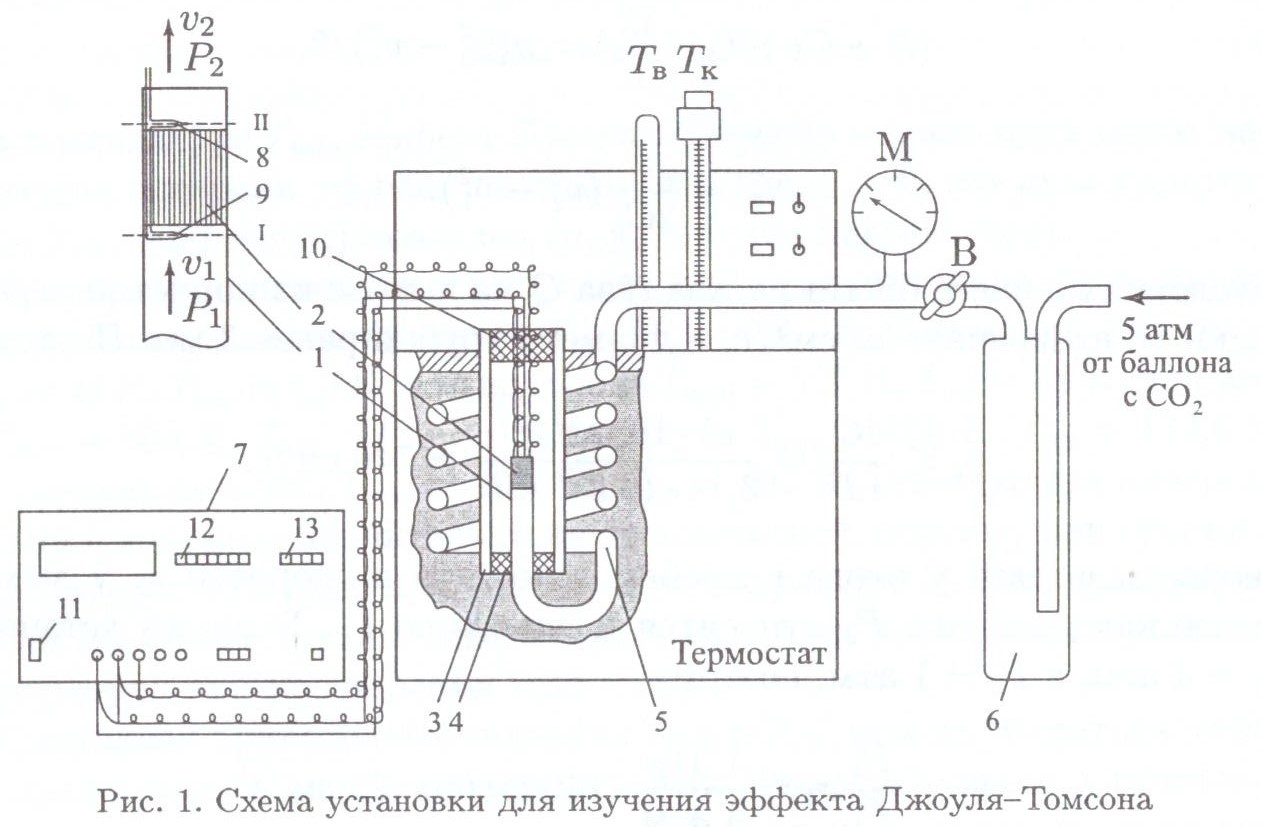
\includegraphics[scale = 1.2]{facility}
		\end{center}
	\end{figure}

	\subsection{Определение коэффициента Джоуля-Томсона}
	
	Проведём измерение зависимости $ \Delta T $ от $ \Delta P $ для разных значений температур. Полученные значения заносим в таблицы. При записи полученных данных также учитываем, что чувствительность термопары медь -- константан зависит от температуры. При вычислении будем использовать следующую формулу: \[ \Delta T = \frac{U}{\alpha}, \] где \[ \alpha_{20^\circ C} = 40,2 \text{ мкВ}/^\circ C, \quad \alpha_{30^\circ C} = 41,1 \text{ мкВ}/^\circ C, \quad \alpha_{50^\circ C} = 42,9 \text{ мкВ}/^\circ C . \]
	
	\begin{table}[H]
		\begin{minipage}{.49\linewidth}
			\centering
			\begin{tabular}{|c|c|c|}
				\hline
				\multicolumn{3}{|c|}{$ T = 22.1 \text{ } ^\circ C $} \\ \hline
				$ \Delta P $, атм &  $ U $, мВ &  $ \Delta T $, K  \\
				\hline
				4 & 0.141 & 3.46 \\ \hline
				3.5 & 0.118 & 2.90 \\ \hline
				3 & 0.096 & 2.36 \\ \hline
				2 & 0.058 & 1.43 \\ \hline
			\end{tabular}
		\end{minipage}
		\begin{minipage}{.49\linewidth}
			\centering
			\begin{tabular}{|c|c|c|}
				\hline
				\multicolumn{3}{|c|}{$ T = 30.1 \text{ } ^\circ C $} \\ \hline
				$ \Delta P $, атм &  $ U $, мВ &  $ \Delta T $, K  \\
				\hline
				4 & 0.134 & 3.30 \\ \hline
				3.5 & 0.112 & 2.78 \\ \hline
				3 & 0.089 & 2.21 \\ \hline
				2 & 0.055 & 1.37 \\ \hline
			\end{tabular}
		\end{minipage}
	\end{table}
	\begin{table}[H]
		\begin{minipage}{.49\linewidth}
			\centering
			\begin{tabular}{|c|c|c|}
				\hline
				\multicolumn{3}{|c|}{$ T = 45.1 \text{ } ^\circ C $} \\ \hline
				$ \Delta P $, атм &  $ U $, мВ &  $ \Delta T $, K  \\
				\hline
				4 & 0.109 & 2.56 \\ \hline
				3.5 & 0.089 & 2.09 \\ \hline
				3 & 0.074 & 1.74 \\ \hline
				2.3 & 0.050 & 1.18 \\ \hline
			\end{tabular}
		\end{minipage}
		\begin{minipage}{.49\linewidth}
			\centering
			\begin{tabular}{|c|c|c|}
				\hline
				\multicolumn{3}{|c|}{$ T = 60 \text{ } ^\circ C $} \\ \hline
				$ \Delta P $, атм &  $ U $, мВ &  $ \Delta T $, K  \\
				\hline
				4 & 0.066 & 1.62 \\ \hline
				3.6 & 0.057 & 1.40 \\ \hline
				3.1 & 0.047 & 1.15 \\ \hline
				2.2 & 0.030 & 0.74 \\ \hline
				
			\end{tabular}
		\end{minipage}
		\caption{Экспериментальные данные для разных температур}
	\end{table}
	
	Кроме того, при вычислении $ \Delta T $ погрешность определяем по формуле:  $\sigma_{\Delta T} = \Delta T \dfrac{\sigma_U}{U}$. Систематические погрешности: $\sigma_P = 0.05 \text{ атм},$ $\sigma_U = 0.001 \text{ мВ}.$
	
	По имеющимся данным проведем аппроксимацию зависимости $ \Delta T $ от $ \Delta P $, чтобы определить коэффициент Джоуля-Томсона. На рисунке \ref{ris} изображены графики зависимостей.
	
	\begin{figure}[!h]
		\centering
		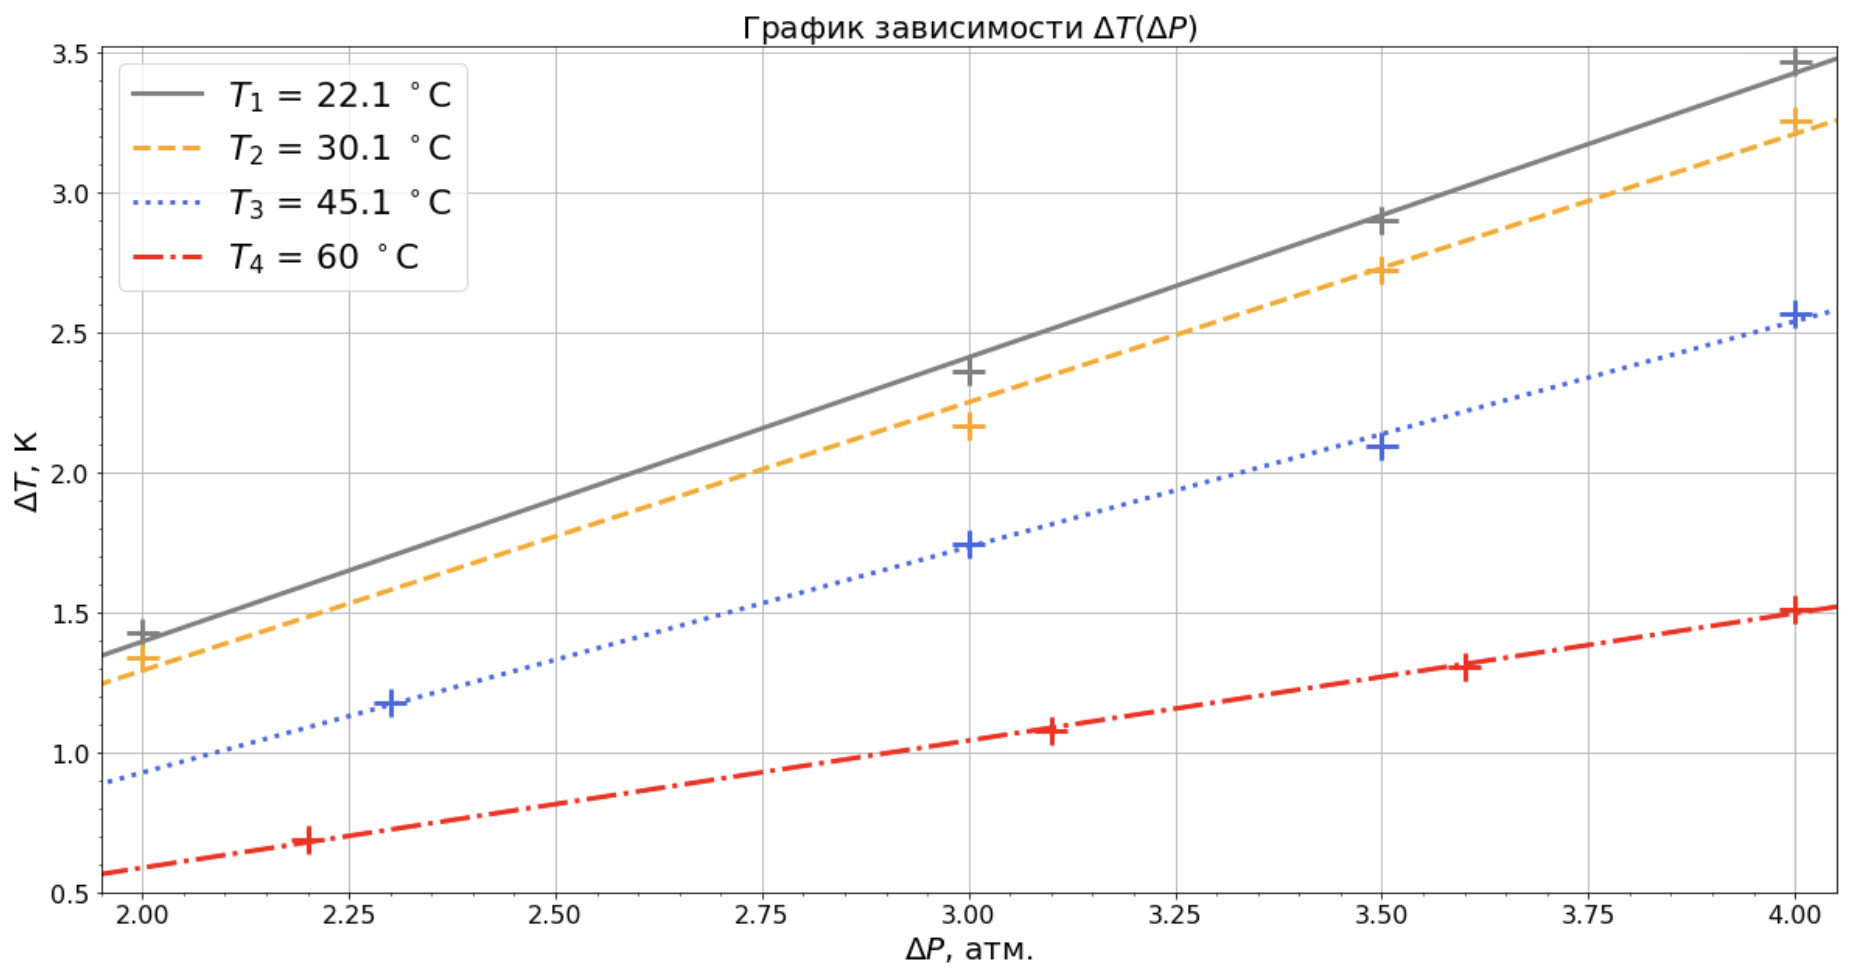
\includegraphics[scale = 0.55]{tp}
		%\caption{График зависимости $T_{н}(Q)$}
		\label{ris}
	\end{figure}
	
	
	Вычислим $ \mu_\text{Д--Т} = \frac{dT}{dP} $, используя метод наименьших квадратов.	
	
	Систематические погрешности оценим по следующим формуле: \[\sigma^\text{сист}_{\mu_\text{Д--Т}} = {\mu_\text{Д--Т}}\sqrt{\varepsilon^2_{\Delta P}+\varepsilon^2_{\Delta T}}.\]
	
	
	Таким образом, полная погрешность измерения определяется следующим соотношением:
	
	\[ \sigma_{\mu_\text{Д--Т}} = \sqrt{(\sigma_{\mu_\text{Д--Т}}^\text{сист})^2 + (\sigma_{\mu_\text{Д--Т}}^\text{случ})^2}.\]
	
	Результаты вычислений заносим в таблицу \ref{tab:my-table}.
	\label{koef}
	\begin{table}[H]
		\centering
		\begin{tabular}{|c|c|c|c|}
			\hline
			$ T $, $ ^\circ C $ & $ \mu_\text{Д--Т} $, К/атм & $ \sigma_{\mu_\text{Д--Т}} $, К/атм & $ \varepsilon $, $ \% $ \\ \hline
			22.1 & 1.015 & 0.053 & 5.2 \\ \hline
			30.1 & 0.9582 & 0.065 & 6.7 \\ \hline
			45.1 & 0.8057 & 0.043 & 5.3 \\ \hline
			60 & 0.488 & 0.023 & 4.7 \\ \hline
		\end{tabular}
		\caption{Результаты измерений $ \mu_\text{Д--Т} $}
		\label{tab:my-table}
	\end{table}
	
	\subsection{Вычисление параметров газа Ван-дер-Ваальса}
	
	Вычислим параметры газа Ван-дер-Ваальса, используя коэффициенты $ \mu_\text{Д--Т} $, полученные в \ref{koef}, для разных пар температур.
	
	Пользуясь формулой \eqref{3}, получим 
	
	\[ \left\{ \begin{aligned}
		a &= \frac{\left(\mu_1 - \mu_2\right)C_PRT_1T_2}{2\left(T_2-T_1\right)}, \\
		b &= \frac{C_P(\mu_2T_2-\mu_1T_1)}{T_1-T_2}. \end{aligned} \right. \]
	
	Погрешности этих вычислений можно оценить используя следующие формулы:~\[ \sigma_a = a\sqrt{\varepsilon^2_{\mu_1-\mu_2}+\varepsilon^2_{T_1}+\varepsilon^2_{T_2}+\varepsilon^2_{T_2-T_1}}, \] \[ \sigma_b=b\sqrt{\varepsilon^2_{\mu_2T_2-\mu_1T_1}+\varepsilon^2_{T_1-T_2}}, \] где \[ \sigma_{x\pm y} =\sqrt{\sigma^2_x+\sigma^2_y}. \]
	
	Для температур 22.1$ ^\circ $C и 30.1$ ^\circ $C, а также для 45.1$ ^\circ $C и 60$ ^\circ $C, вычисляем параметры <<a>> и <<b>> газа Ван-дер-Ваальса. Результаты вычислений заносим в таблицу \ref{tab:a-b}.
	
	\begin{table}[H]
		\centering
		\begin{tabular}{|c|c|c|c|c|c|c|}
			\hline
			$ T $, $ ^\circ C $ & $ a $, $\displaystyle \frac{\text{Па}\cdot\text{м}^6}{\text{моль}^2} $ &$ \sigma_a $, $\displaystyle \frac{\text{Па}\cdot\text{м}^6}{\text{моль}^2} $ & $ \varepsilon_a $, \% & $ b\cdot10^{-4} $, $ \displaystyle\frac{\text{м}^3}{\text{моль}} $ & $ \sigma_b \cdot 10^{-4} $, $\displaystyle \frac{\text{м}^3}{\text{моль}} $ & $ \varepsilon_b $, \% \\ \hline
			30.1 -- 22.1 & 0.97 & 1.46 & 150 & 4.16 & 7.57 & 182 \\ \hline
			45.1 -- 30.1 & 1.49 & 0.76 & 51.1 & 8.33 & 5.26 & 63.1 \\ \hline
			60 -- 45.1 & 3.43 & 0,55 & 16.1 & 23.0 & 5.59 & 24.3 \\ \hline
		\end{tabular}
		\caption{Результаты измерения параметров газа Ван-дер-Ваальса}
		\label{tab:a-b}
	\end{table}
	
	Сверим полученные результаты с табличными. Согласно справочнику для углекислого газа \[ a = 0,36 \text{ } \frac{\text{Па}\cdot\text{м}^6}{\text{моль}^2}, \] \[ b = 0,42\cdot 10^{-4} \text{ }\frac{\text{м}^3}{\text{моль}}. \]
	
	Полученные данные значительно отличаются от табличных. Про причины такого различия сказано в выводе.
	
	\subsection{Вычисление температуры инверсии}
	
	Используя формулу $T_\text{инв} = 27\backslash4T_\text{кр}$, по полученным параметрам газа Ван-дер-Ваальса вычислим $ T_\text{инв} $. Также оценим погрешность по следующей формуле:
	
	\[ \sigma_{T_\text{инв}} = T_\text{инв}\sqrt{\varepsilon^2_a+\varepsilon_b^2}. \]
	
	Результаты вычислений занесём в таблицу \ref{tab:temp}.
	
	\begin{table}[H]
		\centering
		\begin{tabular}{|c|c|c|c|}
			\hline
			$ T $, $ ^\circ C $ & $ T_\text{инв} $, $ ^\circ $К & $ \sigma_{T_\text{инв}} $, $ ^\circ $К & $ \varepsilon $, \% \\ \hline
			30-20 & 489 & 396 & 81 \\ \hline
			50-30 & 485 & 219 & 45 \\ \hline
		\end{tabular}
		\caption{Результаты вычисления температуры инверсии}
		\label{tab:temp}
	\end{table}
	
	Для углекислого газа, согласно справочнику  \[ T_\text{инв} = 2053 \text{ K}.\]
	
	Полученные результаты снова сильно отличаются от табличных.
	
	\section{Обсуждение результатов и выводы}
	
	В ходе выполнения работы мы:
	
	\begin{itemize}
		\item экспериментальным методом измерили коэффициенты газа Ван-дер-Ваальса <<a>> и <<b>>;
		\item вычислили $ T_\text{инв} $ для углекислого газа.
	\end{itemize}
	
	В ходе работы мы получили значения, очень сильно отличающиеся от табличных. Погрешность вычисления параметров газа Ван-дер-Ваальса составила десятки процентов. Такая большая ошибка может говорить нам о неприменимости уравнения Ван-дер-Ваальса в условия лабораторной работы. Действительно, это уравнение используется лишь для качественного описания процессов, происходящих с реальными газами. Количественный подход к этому уравнению неприменим.
	
	Также для увеличения точности измерений можно использовать более точные методы измерения температуры. Повысить точность необходимо как у термостата, так и у вольтметра, т.к. температура на них колебалась на протяжении эксперимента, несмотря на то, что условия оставались неизменными.
	
\end{document}